\documentclass[11pt,a4paper]{article}
\usepackage[greek]{babel}
\usepackage{ucs}
\usepackage[utf8x]{inputenc}
\usepackage{amsmath}
\usepackage{amsfonts}
\usepackage{amssymb}
\usepackage{setspace}
\usepackage{makeidx}
\usepackage{graphicx}
\usepackage{fancyhdr}
\usepackage{paralist}
\pagestyle{fancy}
\usepackage[a4paper]{geometry}
\author{Κοκοβίδης Συμεών 61/13}
\title{ Τμήμα Οργάνωσης \& Διοίκησης επιχειρήσεων \\ Μαθηματικά για Διοίκηση Επιχειρήσεων Ι \\ Πρώτη εργασία στο \LaTeX}
\setlength{\parindent}{0pt} % gia na min dimiourgei esoxes ka8e fora pou allazw 
\everymath{\displaystyle} % gia na min mikrainei tipota
\begin{document}
\maketitle
\onehalfspacing

\textbf{15. ΟΜΑΔΟΠΟΙΗΣΗ ΤΩΝ ΠΑΡΑΤΗΡΗΣΕΩΝ } \newline 
\textbf{ΑΣΚΗΣΗ 1} Εξετάσαμε ορισμένα δρομολόγια ενός οργανισμού σιδηροδρόμων ως προς τον χρόνο (σε \textlatin {min}) που καθυστέρησαν. Τα αποτελέσματα φαίνονται στον παρακάτω πίνακα:


\begin{figure}[hbtp]
\begin{center}
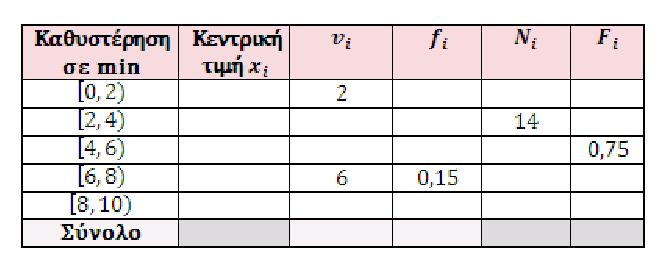
\includegraphics[width=0.6\textwidth, scale=0.5]{1.eps}
\end{center}
\end{figure}


\textbf{α)} Να συμπληρώσετε τον παραπάνω πίνακα  \\
\\
\textbf{β)} Να κατασκευάσετε  το ιστόγραμμα συχνοτήτων και το αντίστοιχο πολύγωνο. \\
\\
\textbf{γ)} Να κατασκευάσετε το ιστόγραμμα αθροιστικών σχετικών συχνοτήτων επί της εκατό και το αντίστοιχο πολύγωνο.\\
\\
\textbf{δ)} Να βρείτε το ποσοστό \% των δρομολογίων που καθυστέρησαν:

\begin{inparaenum}[i.]\itemsep2pt
\item   το πολύ 3 \textlatin{min}.
\item τουλάχιστον 5 \textlatin{min}.
\end{inparaenum}\\

\newpage 

\textbf {ΑΣΚΗΣΗ 2}  Δίνεται ο παρακάτω πίνακας κατανομής συχνοτήτων της μεταβλητής Χ.\\

\begin{figure}[hbtp]
\begin{center}
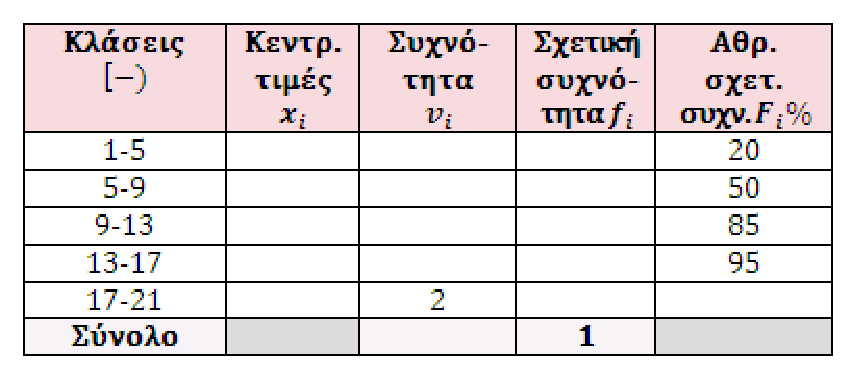
\includegraphics[width=0.6\textwidth, scale=0.5]{2.eps}
\end{center}
\end{figure}


\textbf{α)} Να γράψετε στο τετράδιό σας συμπληρωμένο τον παραπάνω πίνακα.\\
\\
\textbf{β)} Να κατασκευάσετε  το ιστόγραμμα αθροιστικών σχετικών συχνοτήτων επί τοις εκατό και το αντίστοιχο πολύγωνο.\\\\
\textbf{γ) }Να βρείτε το ποσοστό \% των παρατηρήσεων που έχουν τιμές από 4 έως 13. \\\\


\textbf{ΑΣΚΗΣΗ 3}  Στα σχολεία ενός δήμου υπηρετούν συνολικά 100 εκπαιδευτικοί. Ο συνολικός χρόνος υπηρεσίας των εκπαιδευτικών δίνεται από τον παρακάτω πίνακα: \\

\begin{figure}[hbtp]
\begin{center}
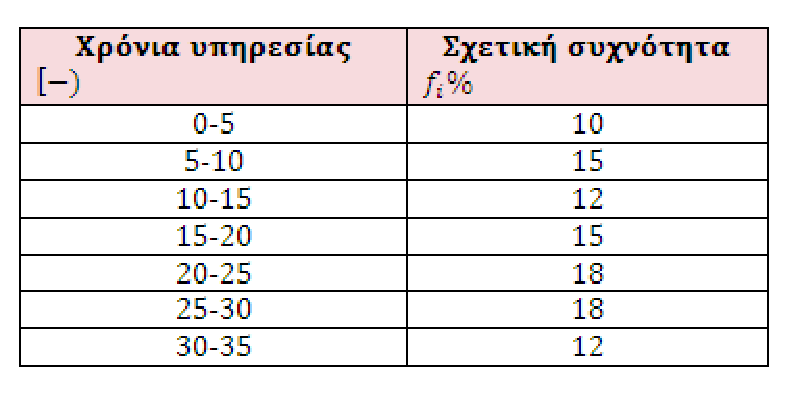
\includegraphics[width=0.6\textwidth, scale=0.5]{3.eps}
\end{center}
\end{figure}

\textbf{α)} Πόσοι εκπαιδευτικοί έχουν τουλάχιστον 15 χρόνια υπηρεσίας\; \\\\
\textbf{β)} Με την προυπόθεση ότι κάθε εκπαιδευτικός θα συνταξιοδοτηθεί όταν συμπληρώσει 35 χρόνια: 
\begin{inparaenum}[i.]\\ %\usepackage{paralist}%
\item πόσοι εκπαιδευτικοί θα συνταξιοδοτηθούν μέσα στα επόμενα 12,5 χρόνια; Να δικαιολογήσετε την απάντηση σας. \\
\item Πόσοι συνολικά εκπαιδευτικοί πρέπει να προσληφθούν μέσα στα επόμενα πέντε χρόνια, ώστε ο αριθμός των εκπαιδευτικών που υπηρετούν στα σχολεία του δήμου να παραμένει ο ίδιος; Να δικαιολογήσετε την απάντησή σας. \\
\end{inparaenum}


\textbf{ΑΣΚΗΣΗ 4} Το βάρος των αποσκευών καθενός εκ των 80 επιβατών μιας πτήσης κάποιας αεροπορικής εταιρίας είναι τουλάχιστον 11 κιλά αλλά μικρότερο από 26 κιλά. Γνωρίζουμε ότι 8 επιβάτες έχουν αποσκευές με βάρος μικρότερο από 14 κιλά, το 30\% των επιβατών έχει αποσκευές με βάρος μικρότερο από 17 κιλά, 48 επιβάτες έχουν αποσκευές με βάρος μικρότερο από 20 κιλά και 15\% των επιβατών έχει αποσκευές μα βάρος τουλάχιστον 23 κιλά.\\

\textbf{α) }Να παρασταθόυν τα δεδομένα σε έναν πίνακα συχνοτήτων ($ν_i$,$N_i$,$f_i$\%,$F_i$\%).\\
\textbf{β)} Κάθε επιβάτης δικαιούται να μεταφέρει αποσκευές με βάρος μικρότερο των 20 κιλών, διαφορετικά έχει πρόσθετη οικονομική επιβάρυνση. Να βρείτε τι ποσοστό από τους 80 επιβάτες της πτήσης έχει πρόσθετη οικονομική επιβάρυνση.\\
\textbf{γ)} Να βρεθούν οι γωνίες των αντίστοιχων κυκλικών τομέων του κυκλικού διαγράμματος σχετικών συχνοτήτων, για τα δεδομένα του προβλήματος.\\


\textbf{ΑΣΚΗΣΗ 5 }Οι βαθμοί φοιτητών στο μάθημα της Στατιστικής ομαδοποιήθηκαν σε 5 κλάσεις ίσου πλάτους. Το πολύγωνο αθροιστικών συχνοτήτων, φαίνεται στο σχήμα που ακολούθει.

\begin{figure}[hbtp]
\begin{center}
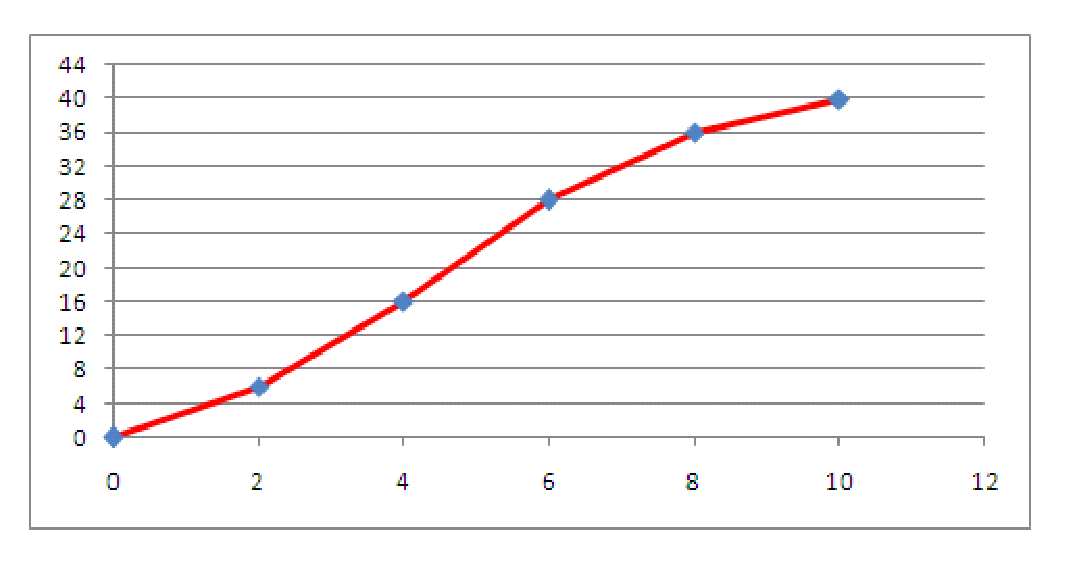
\includegraphics[width=0.6\textwidth, scale=0.5]{5.eps}
\end{center}
\end{figure}

\textbf{α) }Να βρείτε το πλήθος ν των φοιτητών.\\
\textbf{β) }Να κατασκευάσετε τον πίνακα κατανομής $ν_i$,$f_i$,$N_i$,$F_i$.\\
\textbf{γ) }Να κατασκευάσετε το ιστόγραμμα και το πολύγωνο σχετικών συχνοτήτων επί τοις εκατό.\\
{\small \textbf{δ) }Να βρείτε πόσοι φοιτητές δεν πέρασαν το μάθημα Στατιστικής (έγραψαν βαθμό μικρότερο του 5.)\\}

\underline{\textbf{ΑΠΑΝΤΗΣΕΙΣ}}\\
\textbf{ΑΣΚΗΣΗ 1 (16.10) \\
α)} Συμπληρώνουμε τον πίνακα ως εξής:\\

\begin{figure}[hbtp]
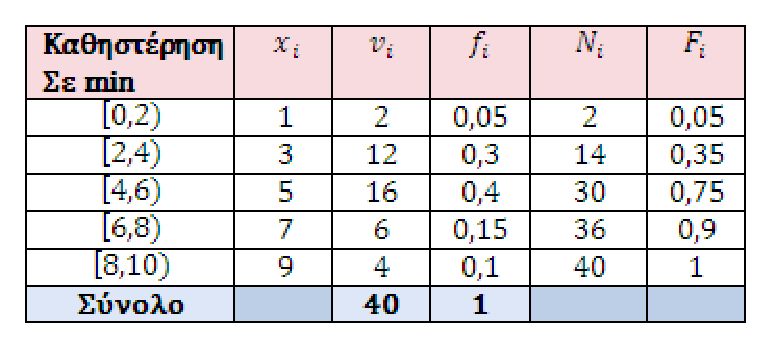
\includegraphics[width=0.6\textwidth, scale=0.5]{A1.eps}
\end{figure}

\textbf{β)}Καθυστέρηση (σε \textlatin{min}) \\
$-2-\nu_i$\\
$0-\nu_i2$\\
$2-\nu_i2$\\
$4-\nu_i12$\\
$6-\nu_i16$\\
$8-\nu_i6$\\
$10-\nu_i4$\\
$12-\nu_i$\\


\textbf{ γ)  }Καθυστέρηση (σε \textlatin{min})
$0-F_i\%5$\\
$2-F_i\%5$\\
$4-F_i\%35$\\
$6-F_i\%75$\\
$8-F_i\%90$\\
$10-F_i\%100$\\

\textbf{ δ}) i) $20\%$  ii)  $ 45\%$\\
\newpage

\textbf{ ΑΣΚΗΣΗ 2 (16.11)    }
\textbf{α}) Συμπληρώνουμε τον πίνακα ως εξής:

\begin{figure}[hbtp]
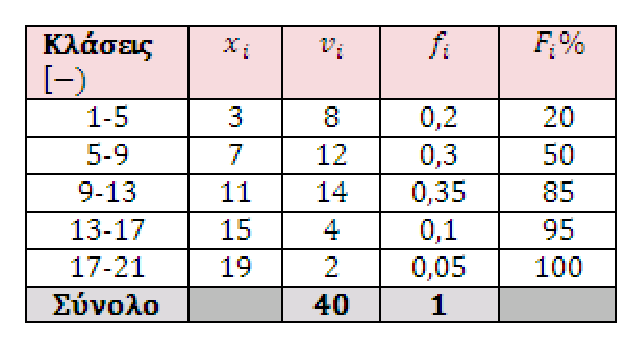
\includegraphics[width=0.6\textwidth, scale=0.5]{A2.eps}
\end{figure}

\textbf{ β)  }Κλάσεις \\
$1-F_i\%20$\\
$5-F_i\%50$\\
$9-F_i\%85$\\
$13-F_i\%95$\\
$17-F_i\%100$\\
$21-F_i\%$\\

\textbf{ γ) }$70\%$\\

\textbf{ ΑΣΚΗΣΗ 3 (16.14) }
\textbf{α}) Από τον πίνακα παρατηρούμε ότι το ποσοστό των καθηγητών που έχουν τουλάχιστον 15 χρόνια υπηρεσίας είναι $(15+18+18+12)\%=63\%$ \\
Εφόσον ο συνολικός αριθμός των εκπαιδευτικών είναι 100, ο αριθμός των καθηγητών με τουλάχιστον 15 χρόνια υπηρεσίας είναι 63.\\
\textbf{ β) }
\begin{enumerate}[i]\item Οι εκπαιδευτικοί που θα πάρουν σύνταξη μέσα στα επόμενα12,5 χρόνια είναι όσοι έχουν τουλάχιστον 22,5 χρόνια υπηρεσίας. Δηλαδή το ποσοστό είναι: \begin{center} $(\frac{18}{2}+18+12)\%=39\%$ \end{center}
Συνεπώς το πλήθος των εκπαιδευτικών είναι 39.
\item Τα επόμενα πέντε χρόνια πρέπει να προσληφθούν συνολικά τόσοι εκπαιδευτικοί όσοι θα συνταξιοδοτηθούν. Δηλαδή όσοι ανήκουν στην κλάση [30,35), άρα 12 εκπαιδευτικοί.
\item 45\%
\end{enumerate}

\newpage

\textbf{ ΑΣΚΗΣΗ 4 (16.16)   } 
\textbf{α}) Ο ζητούμενος πίνακας είναι ο παρακάτω:\\

\begin{figure}[hbtp]
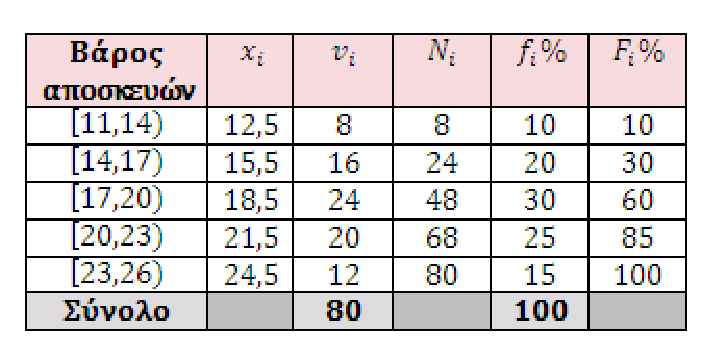
\includegraphics[width=0.6\textwidth, scale=0.5]{A4.eps}
\end{figure}

\textbf{ β})Το ποσοστό είναι ίσο με $100\%-F_3\%=40\%$ \\

\textbf{γ})$α_1=36^{\circ}, α_2=72^{\circ},α_3=108^{\circ},α_4=90^{\circ}$ και $α_5=54^{\circ}$\\


\textbf{ ΑΣΚΗΣΗ 5 (16.20)   } $v=40.$\\
\textbf{α})
\textbf{ β)  }Κατασκευάζουμε τον πίνακα ως εξής:\\

\begin{figure}[hbtp]
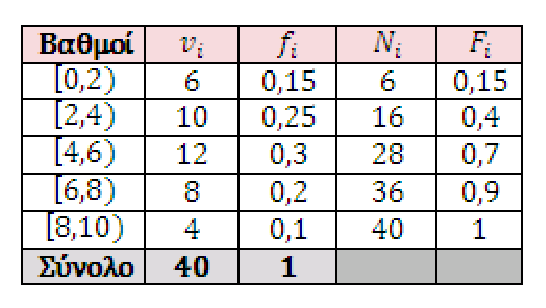
\includegraphics[width=0.6\textwidth, scale=0.5]{A5.eps}
\end{figure}

\textbf{ γ})\\\\
\textbf{δ}) 22.\\




\end{document}